\section{Experiments}



\begin{table*}[t]
\caption{Experimental Results on math reasoning benchmarks(Accuracy \%).}
\centering
% \small
\setlength{\tabcolsep}{4pt}
\begin{tabular}{lcccc}
\toprule
Model & AIME2025 & BeyondAIME & HMMT Nov 2025 & IMOAnswerBench  \\
\midrule
% Qwen3-30B-A3-Thinking-2507 & 85.0 &  \\
% Qwen3-235B-A22-Thinking-2507 & 92.3 & \\
Claude-Sonnet-4.5 & 87.0 & 62.0 & 81.7 & 65.8 \\
GPT-5 High & 94.6 & 74.0 & 89.2 & 76.0 \\
% GLM-4.5 & 91.0 & \\
GLM-4.7 & 95.7 & - & 93.5 &  82.0\\
\midrule
Qwen3-30B-A3B  \\
\quad w/ python & 14.6 & 10.5 & 17.3 & 7.8 \\
\quad w/o python & 85.0 & 63.0 & 76.7 & 55.3 \\
\quad SFT (w/ python) & 80.4 & 53.3 & 75.2 & 53.3 \\
\quad SFT (w/o python) & 14.6 & 46.8 & 17.3 & 42.0 \\
 % \midrule
\quad GRPO (w/ python) & 84.2 & 54.8 & 76.0 &  55.8\\
%  Qwen3-30B-A3B-GRPO (w/ DIS) & 94.2 & 71.5 & 86.7 & 71.3\\
  
  % Qwen3-30B-A3B VAPO & 79.79 & 55.25 & 74.58 & 77.50 & 54.00 \\
 % Qwen3-30B-A3B RunningMean & 91.25 & 69.00 & 82.29 & 83.12 & 69.75 \\
 % \model (ours) & 95.6 & 75.5 & 90.8 & 73.5 \\
 \midrule
Qwen3-30B-A3B \\
\rowcolor{saoRowGray}
\quad  \model (ours) & \textbf{97.3} & \textbf{74.8} & \textbf{88.3} & \textbf{74.0} \\
\quad  - \textit{SAO (w/ DIS only)} & 94.2 & 71.5 & 86.7 & 71.3\\
\quad - \textit{GRPO (+ DIS)} & 93.5 & 70.8 & 84.0 & 70.0 \\

\bottomrule
\end{tabular}
\label{tab:main_results}
\end{table*}


\begin{table*}[t]
    \centering
    \caption{Experimental Results  on SWE-Bench Verified (Accuracy \%).}
    \begin{tabular}{l|c}
    \toprule
     Model    & Accuracy (\%) \\
    \midrule
    Qwen3-30B-A3B    &  23.0 \\
    + GRPO (w/ DIS)     & 27.0 \\
\rowcolor{saoRowGray}
    + \model (ours) & 29.8 \\
    \bottomrule
    \end{tabular}
    \label{tab:swe_bench}
%\vspace{-2mm}
\end{table*}
%-Thinking-2507 

\begin{figure*}[t]
\centering
  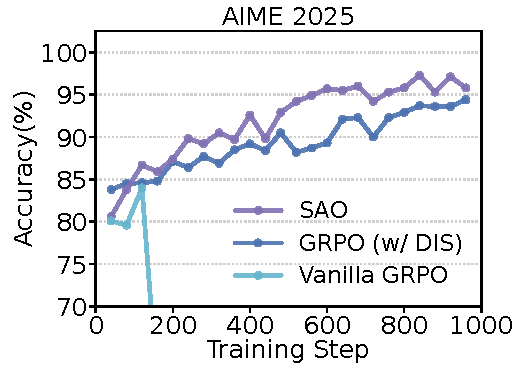
\includegraphics[width=0.32\textwidth]{figures/main_result_aime.pdf}
\hfill
  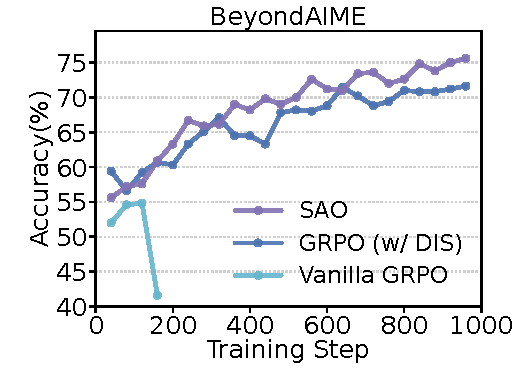
\includegraphics[width=0.32\textwidth]{figures/main_result_beyondaime.pdf}
\hfill
  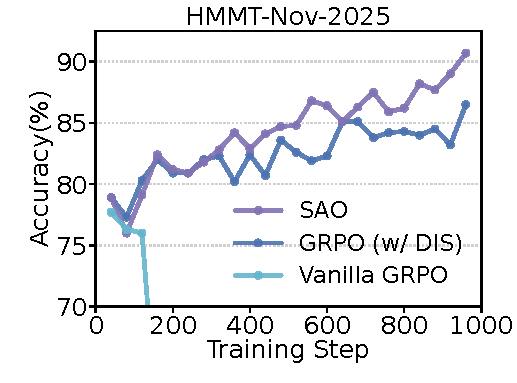
\includegraphics[width=0.32\textwidth]{figures/main_result_hmmtnov.pdf}
\caption{Performance comparison between \model and GRPO (w/ DIS) during training. It can be observed that \model almost consistently outperforms the optimized GRPO during the training process on different benchmarks. 
% Results on the remaining benchmarks are included in Appendix\ref{}.
}
\label{fig:main_results}
\vspace{-4mm}
\end{figure*}



\subsection{Experimental Setup}
\vpara{Training Details.}
% For all experiments, the policy and critic are initialized from a Qwen3-30B-A3B-Thinking-2507 model. 
For math reasoning with Python, we finetune Qwen3-30B-A3B-Thinking-2507~\citep{yang2025qwen3} for 3 epochs on Tool-Integrated Reasoning (TIR) data produced by GPT-OSS-120B~\citep{openai2025gptoss120bgptoss20bmodel} and use the finetuned model to initialize the policy and value model. TIR requires the model to interleave natural-language math reasoning with Python tool calls.

For RL of agentic reasoning, we employ a batch size of 128, a group size of 1, and a max-length of 128k tokens. The policy is optimized with a learning rate of $1 \times 10^{-6}$, with a token clipping of $\epsilon_{\text{low}}=0.3$, $\epsilon_{\text{high}}=5.0$. 
% For advantage estimation,
We adopt a length-adaptive GAE~\citep{yue2025vapo} with $\lambda_{\text{policy}} = 1 - \frac{1}{\alpha l}$ and $\alpha = 1.5$. The value model is trained with a learning rate of $5 \times 10^{-6}$, $\lambda_{\text{critic}} = 1$, and a 10-step warmup period. We set the $K=2$ for faster value update for the value model, performing two value model updates per batch. For GRPO variants, each training batch contains 16 prompts with 8 rollout samples per prompt, yielding the same batch size of 128.
For the RL of coding agent, we directly use Qwen3-30B-A3B-Thinking-2507 for training and keep almost all the hyperparameters the same as TIR, except for $\epsilon_{\text{low}}=0.8$ and $\epsilon_{\text{high}}=3.0$. For SWE-Bench Verified, we use OpenHands as the scaffold, with a maximum of 300 interaction turns and a 128k-token context budget.

\vpara{Evaluation.} We evaluate \model on four math reasoning benchmarks including AIME2025, BeyondAIME\citep{bytedance_seed_2025_beyondaime}, 
% \HMMT Feb 2025\citep{balunovic2025matharena}, 
HMMT Nov 2025\citep{balunovic2025matharena} and IMOAnswerBench\citep{luong-etal-2025-towards}, reporting Pass@1 accuracy. All evaluations use top-$p=1.0$, temperature $1.0$, and a maximum generation length of 128k tokens. Math-reasoning evaluations allow up to 50 turns to support extensive reasoning and tool calls, while SWE-Bench Verified evaluations allow up to 300 OpenHands interaction turns. To reduce variance, we report the mean performance across 16 evaluation runs for AIME2025 / HMMT / IMOAnswerBench and 4 runs for BeyondAIME.



% \begin{table*}[t]
% \caption{Experimental Results on math reasoning benchmarks. We report Accuracy(\%) for all datasets.}
% \centering
% \begin{tabular}{lccccccc}
% \toprule
% Model & AIME2025 & BeyondAIME & HMMT Nov 2025 & HMMT Feb 2025 & IMOAnswerBench  \\
% \midrule
% % Qwen3-30B-A3-Thinking-2507 & 85.0 &  \\
% Qwen3-235B-A22-Thinking-2507 & 92.3 & \\
% Claude-sonnet-4.5 & 87.0 & 62.0 & 81.7 & 79.2 & 65.8 \\
% GPT-5 High & 94.6 & 74.0 & 89.2 & 88.3 & 76.0 \\
% % GLM-4.5 & 91.0 & \\
% GLM-4.7 & 95.7 & - & 93.5 & 97.1 & 82.0\\
% \midrule
% Qwen3-30B-A3B (w/ python) & 14.6 & 10.5 & 17.3 & 12.3 & 7.8 \\
% Qwen3-30B-A3B (w/o python) & 85.0 & 63.0 & 76.7 & 70.4 & 55.3 \\
% Qwen3-30B-A3B-SFT (w/ python) & 80.4 & 53.3 & 75.2 & 73.1 & 53.3 \\
% Qwen3-30B-A3B-SFT (w/o python) & 14.6 & 46.8 & 17.3 & 12.3 & 42.0 \\
%  \midrule
%  Qwen3-30B-A3B-GRPO & 84.17 & 54.75 & 76.04 & 71.46 & 55.75\\
%  Qwen3-30B-A3B-GRPO (w/ DIS) & 94.17 & 71.50 & 86.67 & 88.96 & 71.25\\
%   % Qwen3-30B-A3B VAPO & 79.79 & 55.25 & 74.58 & 77.50 & 54.00 \\
%  % Qwen3-30B-A3B RunningMean & 91.25 & 69.00 & 82.29 & 83.12 & 69.75 \\
%  \model (ours) & 95.63 & 75.50 & 90.83 & 89.58 & 73.50 \\
% \bottomrule
% \end{tabular}
% \label{tab:main_results}
% \end{table*}


\subsection{Main Results}
Tables \ref{tab:main_results} and \ref{tab:swe_bench} summarize the performance of baselines and different training strategies. GRPO denotes the standard GRPO with \textit{clip-higher} implementation~\cite{yue2025vapo}, which keeps the latest old policy for importance sampling. GRPO (w/ DIS) denotes using the proposed DIS strategy for GRPO.


% \begin{itemize}[leftmargin=*,itemsep=0pt,parsep=0.2em,topsep=0.3em,partopsep=0.3em]
% \item \textbf{Standard GRPO}: The vanilla GRPO baseline,, which keeps the latest old policy for importance sampling. 

% \item \textbf{GRPO w/ DIS}: A GRPO variant adapted for asynchronous settings. Following our proposed importance sampling mechanism, it utilizes log-probabilities from rollout logs as a behavior proxy to mitigate policy lag.

% \end{itemize}


% \item \textbf{GRPO (Simplified importance sampling)}: A GRPO variant incorporating the icepop-clipping strategy to stabilize policy updates. 
% \item \textbf{RunningMean}: A variant that maintains a sliding window of the 8 most recent rewards for each prompt, using their mean as the baseline for advantage estimation. \end{itemize}

As shown in Tables \ref{tab:main_results} and ~\ref{tab:swe_bench}, \model consistently outperforms all baselines on both agentic reasoning and coding benchmarks. Standard GRPO
% and VAPO 
suffers from a performance collapse at approximately 160
% and 90 
training steps
% , respectively. 
The scores reported for these models represent their final valid performance before collapsing.
% , highlighting the challenge of stabilizing single-rollout RL in complex reasoning tasks without our proposed stabilization mechanisms.
Figure \ref{fig:main_results} illustrates the evaluation performance across training steps of \model compared to vanilla GRPO and GRPO (w/ DIS). Vanilla GRPO tends to quickly collapse, while GRPO with DIS can achieve stable training, demonstrating the effectiveness of DIS. 
In addition, \model and GRPO (w/ DIS) exhibit comparable performance in the initial stage; a distinct performance divergence occurs after approximately 400 training steps, demonstrating the effectiveness and stability of \model.





\subsection{Ablation Studies}
We conduct extensive ablation studies to evaluate the impact of various training configurations on the performance of \model. The results are shown in Table~\ref{tab:ablations}.

\begin{itemize}[leftmargin=*,itemsep=0pt,parsep=0.2em,topsep=0.3em,partopsep=0.3em]
% \item \textbf{Partial Value Pre-training}: To investigate the contribution of pre-training initialization to final performance, we ablate the value pre-training stage by utilizing a reduced $3.2k$-sample corpus and adopting attention freezing, compared to the full-parameter pre-training on $6k$ samples used in \model. Notably, during the subsequent RL stage, this variant also employs attention-freezing strategy as \model, attributing the performance change solely to the quality of value pre-training.
\item \textit{Effects of faster value update}: To ablate the effects of faster value update than the policy model, we conduct experiments where the value model is updated only once per batch (critic-train-epoch=1), as opposed to the two updates per batch employed in \model. 
% \item \textbf{Naive GAE}: This configuration extends the Generalized Advantage Estimation (GAE) calculation across the entire sequence, including observation tokens, whereas the proposed method restricts this computation to model-generated output tokens. 
\item \textit{Full vs. frozen-attention value model.}: To evaluate the impact of attention-freezing during RL, this variant performs full-parameter updates on the value model. 

\item \textit{Vanilla VAPO and single-rollout with Running-mean baseline.} Standard VAPO\citep{yue2025vapo} with length-adaptive GAE and a value-based RL baseline. Besides, a single-rollout baseline that maintains a sliding window of the 8 most recent rewards for each prompt, using their mean as a baseline for advantage estimation to provide a simple alternative to parametric value models.

\end{itemize}

As shown in Table \ref{tab:ablations}, all examined variants exhibit a performance decline relative to the proposed \model, validating the necessity of each design choice. Table~\ref{tab:value_training_ablations} further summarizes the value-training strategy and critic-update settings behind the main value-model ablations. Regarding update frequency, the results indicate that a single update is insufficient for the critic to accurately track rapid policy shifts, leading to less reliable baseline estimations. The full-parameter value-training variant further suggests that frozen-attention updates help regularize critic optimization in complex reasoning tasks.
In addition, the RL with running-mean reward achieves decent performance, but still lags far from our \model, demonstrating the advantage and necessity of a well-trained value model for RL. As for the vanilla VAPO, the training also quickly collapses during training, similar to the vanilla GRPO. 
% For GAE computation, since observation tokens are excluded from value model optimization, their inclusion in the advantage estimation introduces significant noise that destabilizes policy updates. 
% The underperformance of full-parameter value training underscores that updates to the entire critic can lead to distortion of pre-trained representations and less stable reinforcement learning.
% \begin{table}[]
% \caption{}
% \centering
% \begin{tabular}{lcccc}
% \toprule
% Model & AIME2025 & BeyondAIME\\
% \midrule
%  \model & 95.63 & 75.50 \\
%  \midrule
%  % Partial Value Pre-training & 92.50 & 71.50 \\
%  Single Critic Update & 95.00 & 69.75 \\
%  % Naive GAE & & \\
%  Full-Parameter Value Training & 90.62 & 74.50 \\
% \bottomrule
% \end{tabular}
% \label{tab:ablations}
% \end{table}





\begin{figure*}[htbp]
\centering
\subfloat[]{
  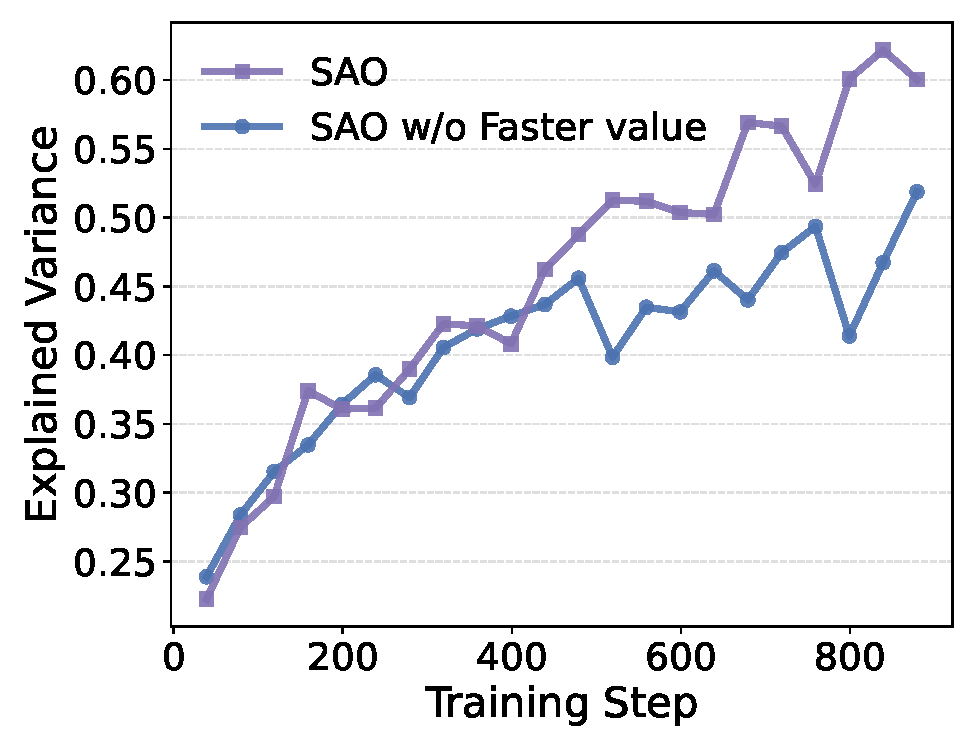
\includegraphics[width=0.32\textwidth]{figures/main_vs_criticonce_ev.pdf}
}
\hfill
\subfloat[]{
  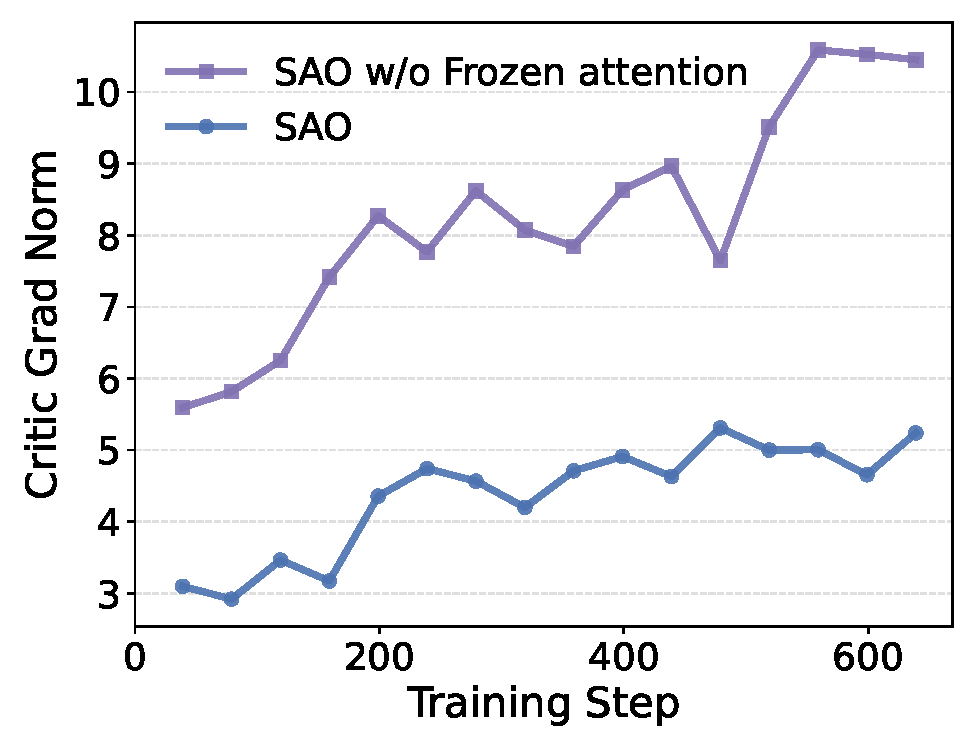
\includegraphics[width=0.32\textwidth]{figures/main_vs_fullparam_criticgradnorm.pdf}
}
\hfill
\subfloat[]{
  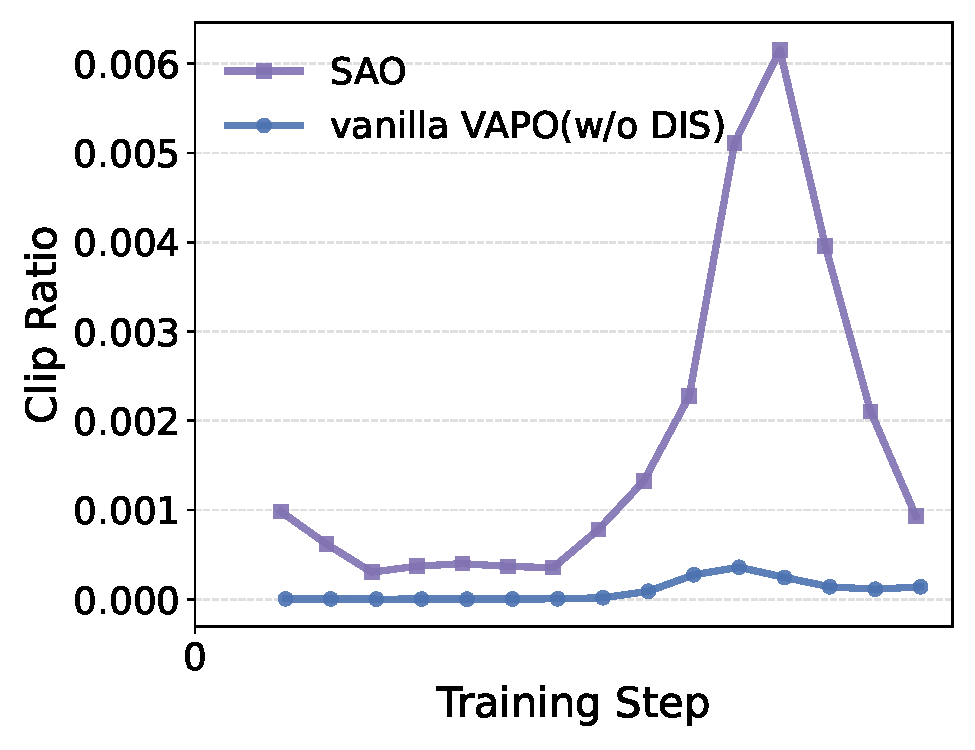
\includegraphics[width=0.32\textwidth]{figures/grpo_vs_grpobasic_clipratio.pdf}
}
% \caption{}
\caption{
Training dynamics of asynchronous single-rollout RL.
(a) Explained Variance for \model and a single-critic-update baseline.
(b) Critic gradient norm during value training under full-parameter optimization and frozen-attention optimization used in \model.
(c) Token-level clip ratio during training for \model with the proposed DIS and the VAPO baseline.
}
\label{fig:training_dynamics}
\end{figure*}


%\subsection{Analysis}
\subsection{Training Dynamics}
We analyze the training dynamics of \model to understand how it facilitates training stability.

\vpara{Effects of Faster Value Update.} Figure \ref{fig:training_dynamics}(a) illustrates Explained Variance comparison between \model and the single-critic-update baseline during training. Explained Variance assesses the alignment between the predicted values $V(s)$ and the ground-truth returns $R$, defined as $EV = 1 - \frac{\text{Var}(R - V(s))}{\text{Var}(R)}$. 
\model demonstrates significantly higher explained variance after approximately 400 training steps, indicating faster value convergence and better alignment with policy distribution.

\vpara{Gradient of Critic Models.} We examine the impact of freezing attention parameters in value training. As shown in Figure \ref{fig:training_dynamics}(b), full-parameter value training exhibits significantly larger critic gradient norms, suggesting unstable optimization dynamics. In contrast, the frozen-attention strategy maintains lower and smoother gradient norms, implying improved numerical stability.

\vpara{Clipped Tokens.} Figure \ref{fig:training_dynamics}(c) monitors the token-level clip ratio of \model applying our proposed DIS strategy and the standard VAPO baseline without it. While VAPO maintains a near-zero clip ratio, it fails to effectively gate divergent off-policy updates, leading to a rapid training collapse at approximately 90 steps. 
% In contrast, \model maintains a dynamic clip ratio, demonstrating that our DIS effectively identifies and suppresses excessive policy shifts, thereby maintaining the trust region during asynchronous updates.

% \subsubsection{Analysis on Value Model}
% To ensure a fair comparison and evaluate the generalization ability of the value model, all following analyses are conducted on test set BeyondAIME. To validate the effectiveness of value pre-train and analyze critic model behavior, we evaluate the critic based on the following three metrics:
% \begin{itemize}
%     \item \textbf{Explained Variance (EV):} This metric assesses the alignment between the predicted values $V(s)$ and the ground-truth returns $R$, defined as $EV = 1 - \frac{\text{Var}(R - V(s))}{\text{Var}(R)}$. A higher EV indicates more accurate capture of the return distribution.
    
%     \item \textbf{Value Margin:} To measure the model's discriminative capacity, we calculate the mean value difference between positive samples ($S^+$) and negative samples ($S^-$) for each prompt: $\Delta V = \mathbb{E}_{s \in S^+} [V(s)] - \mathbb{E}_{s \in S^-} [V(s)]$. A larger margin reflects a stronger ability to distinguish between high- and low-quality responses.

%     \item \textbf{Value-Accuracy Correlation:} We compute the Pearson correlation coefficient between the average predicted value within a reasoning step and the success rate of rollouts initiated from the end of that step. Formally, for each step $i$, we calculate the mean value $\bar{V}_i = \frac{1}{N_i} \sum_{t \in \text{step}_i} V(s_t)$ and its correlation with the empirical pass rate $P(\text{success} | s_{i, \text{end}})$. A high correlation indicates that the value model serves as an accurate proxy for the expected objective achievement throughout the reasoning process.
% \end{itemize}
% Figure\ref{fig:critic_metrics} compares the proposed full-parameter critic (6k samples) against the Expert-Only variant (3.2k samples, Section\ref{}). As value pre-training progresses, the full-parameter critic consistently achieves higher EV, a wider value margin, and a stronger Pearson correlation with rollout success rates. Collectively, these three metrics serve as robust proxies for critic quality, demonstrating that scaling both data volume and trainable parameters leads to more precise return modeling, enhanced discriminative capacity, and more accurate fitting of pass rates. This enhanced quality provides the accurate reward signals required for effective policy guidance, directly explaining the superior performance of \model over the Expert-Only ablation.

% \begin{figure*}[htbp]
% \centering
% \subfloat[]{
%   \includegraphics[width=0.32\textwidth]{figures/ev.pdf}
% }
% \hfill
% \subfloat[]{
%   \includegraphics[width=0.32\textwidth]{figures/ev.pdf}
% }
% \hfill
% \subfloat[]{
%   \includegraphics[width=0.32\textwidth]{figures/ev.pdf}
% }
% \caption{}
% \label{fig:critic_metrics}
% \end{figure*}


\begin{table*}[ht]
\caption{Ablation results of value model training strategy and critic update frequency. We compare partial parameters, i.e., frozen-attention, with full-parameter value update in RL training, as well as the effectiveness of faster critic updates per policy step. We report Accuracy (\%) for all datasets}
\centering
% \small
\setlength{\tabcolsep}{4pt}
\begin{tabular}{lcccc}
\toprule
 & \makecell{Value Training\\Strategy} & \makecell{Critic Update\\Frequency} & AIME2025 & BeyondAIME \\
\midrule
\model & Frozen Attention & 2 & 97.3 & 74.8 \\
\midrule
Single-step-update & Frozen Attention & 1 & 95.00 & 69.75 \\
Full-Parameter Value Training & Full-Parameter & 2 & 90.62 & 74.50 \\
\bottomrule
\end{tabular}
% \caption{The training dynamics ablation of designs in \model. (a); (b); (c)}
\label{tab:value_training_ablations}
\end{table*}


\begin{table}[ht]
\caption{Ablation results of value model training strategy and critic update frequency. We compare partial parameters, i.e., frozen-attention, with full-parameter value update in RL training, as well as the effectiveness of faster critic updates per policy step. We report Accuracy (\%) for all datasets}
\centering
\begin{tabular}{lcc}
\toprule
  & AIME2025 & BeyondAIME \\
\midrule
\model & 97.3 & 74.8 \\
\midrule
\model w/o Faster value & 95.0 & 69.8 \\
\model w/o Frozen attention  & 90.6 & 74.5 \\
Vanilla VAPO (w/o DIS) & 91.3 & 69.0 \\
Running mean baseline & 79.8 & 55.3 \\
\bottomrule
\end{tabular}
% \caption{The training dynamics ablation of designs in \model. (a); (b); (c)}
\label{tab:ablations}
\vspace{-3mm}
\end{table}


\subsection{Online Learning Simulation}
\vpara{Task Design.} 
% To further evaluate the adaptability of \model, we conduct experiments in an online learning setting. 
In real-world online learning environments, feedback is typically restricted to a single trajectory per prompt. 
This constraint is inherently incompatible with group-based optimization strategies like GRPO, which depend on relative rewards within a sample group for advantage estimation. In contrast, \model utilizes a value-based critic to provide advantage estimation, allowing for effective policy updates from individual trajectories. 

Therefore, we design a simulated online writing task to assess the adaptability of \model in non-stationary environments. 
In this setting, the feedback signal is designed as the language tone of user preference.
Reward criteria are sequentially adjusted to favor three distinct stylistic archetypes: \textit{cute}, \textit{chuunibyou}, and \textit{classical}. 
% This phased configuration enables us to monitor the model's capacity to detect shifts in reward distribution and re-align its policy.

\vpara{Dynamic Reward Assignment.} For reward signal assignment, we employ GLM-4.7\citep{2025glm} as an LLM-based judge to evaluate two primary dimensions: response quality and stylistic adherence. The final reward $r \in \{0, 1\}$ is computed as: $r = r_{\text{quality}} \times r_{\text{style}}$ where $r_{\text{quality}}, r_{\text{style}} \in \{0, 1\}$ denote binary rewards. 

% Throughout training, the system prompt requires the model to select one of three stylistic archetypes. In our actual implementation, this candidate set consists of \textit{cute}, \textit{chuunibyou}, and \textit{academic} during the first two phases, \textit{cute}, \textit{chuunibyou}, and \textit{classical} in the last phase.
Throughout training, the system prompt requires the model to select one stylistic archetype from a pool of four candidates: Academic, Cute, Chuunibyou, and Classical. In our actual experiments, the candidate set consists of \textit{Academic, Cute, Chuunibyou} during the first two phases, and \textit{Classical, Cute, Chuunibyou} in the final phase.
% To facilitate policy bootstrapping during these transitions, we apply a warm-up strategy: for the initial 18 steps of each phase, 50\% of the trajectories are generated using prompts that explicitly specify the target style to initiate policy realignment. 
% During policy updates, all trajectories are re-formatted with standardized selection prompts, decoupling the training signal from explicit instructions. 
% During policy update, we re-format all trajectories with standardized selection-based prompts, thereby decoupling the training signal from the explicit stylistic instructions used during rollout. This procedure ensures that the model learns to adapt its policy based on reward distribution rather than relying on textual guidance.

\vpara{Results.} As illustrated in Figure \ref{fig:writing_eval}, we evaluate the performance of the three candidate linguistic styles of each phase on a held-out test set
% throughout training
. \model demonstrates rapid policy realignment following each reward preference shift, characterized by transitions between stylistic archetypes to maintain adherence to the evolving environmental feedback.

\vpara{Comparison against Running-Mean Baseline.} 
% To address the infeasibility of applying GRPO in a single-rollout configuration,
To better understand the effectiveness of the value model in the online environment, we also adopt the Running Mean Advantage Estimation approach as the baseline. This method approximates the baseline $b$ by tracking a sliding window of the 128 most recent rewards, thereby facilitating advantage computation as $\hat{A} = r - \mathbb{E}[r_{window}]$. By decoupling advantage estimation from intra-prompt sample groups, this setup permits policy optimization in an online, single-rollout context.
% of comparison for \model’s value-based critic.
Figure \ref{fig:writing_training} depicts the evolution of training rewards throughout the online learning process of \model and the Running Mean baseline, where the speed and magnitude of reward recovery following stylistic shifts serve as key indicators of algorithmic adaptability. 
% While both methods achieve online realignment, \model demonstrates superior adaptation ability. 
The Running Mean baseline exhibits a pronounced adaptation lag due to the inertia of its historical window, which remains temporarily biased by rewards from the preceding distribution. In contrast, \model's value-based critic dynamically tracks reward shifts, facilitating rapid recovery and consistently higher convergence levels. This confirms that \model's state-dependent baseline provides the precision necessary for effective alignment in non-stationary environments.

\begin{figure*}[ht]
\centering
\subfloat[We report the accuracy transition of three writing styles---cute, chuunibyou, and classical---on a held-out evaluation set throughout the online training process. Shaded regions indicate phase transitions where the reward preference is switched to favor a different stylistic archetype. \model rapidly suppresses the previously dominant style and realigns its policy to the new target based on environmental feedback.]{
  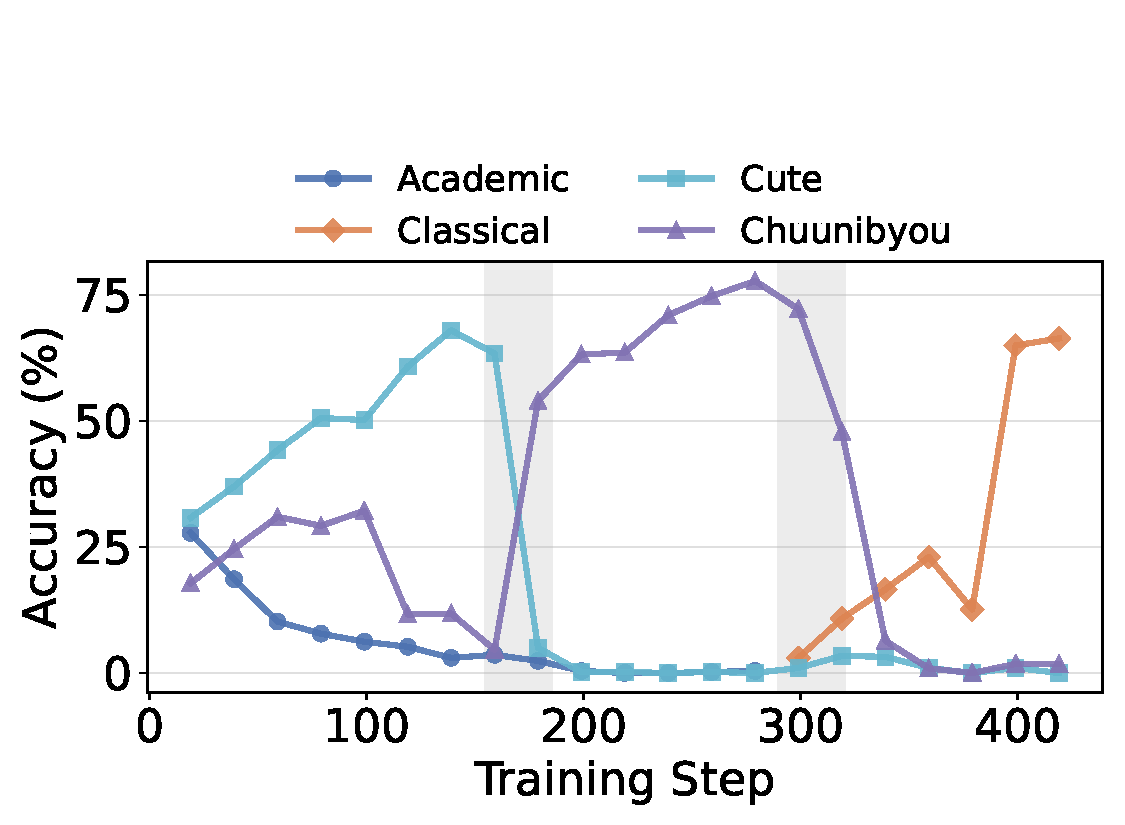
\includegraphics[width=0.48\textwidth]{figures/writing_eval_classicalprompt.pdf}
  \label{fig:writing_eval}
}
\hfill
\subfloat[We compare the evolution of training rewards between \model and a Running Mean Advantage Estimation baseline under single-rollout online learning. Shaded regions denote stylistic reward shifts. While both methods eventually recover after distribution changes, the Running Mean baseline exhibits a pronounced adaptation lag and lower stable performance.]{
  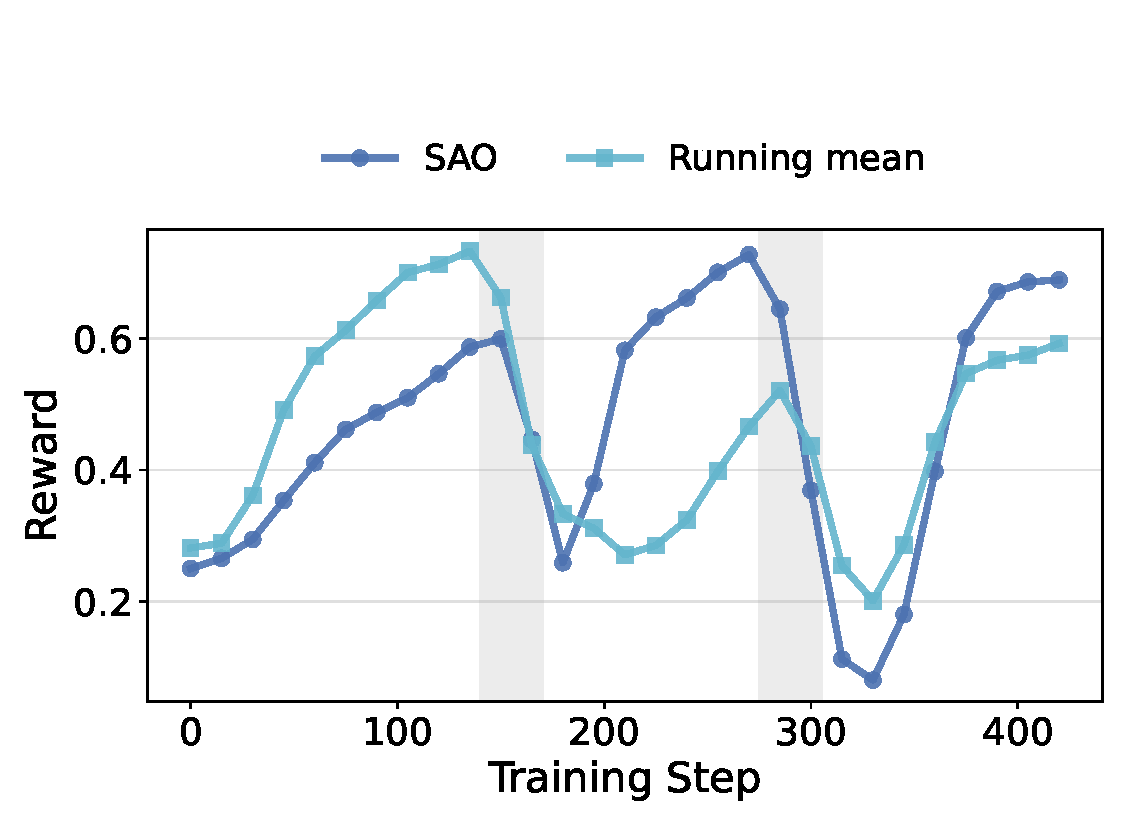
\includegraphics[width=0.48\textwidth]{figures/writing_training_reward.pdf}
  \label{fig:writing_training}
}
\caption{Online learning simulation under changing writing-style preferences.}
\label{fig:writing_online}
\end{figure*}
